%This is the first chapter of the \gls{thesis}.~\cite{Aaboud:2016mmw,Bruning:782076}

\section{Creating Figures}\label{sec:figures}
\begin{figure}[htpb]
 \centering
 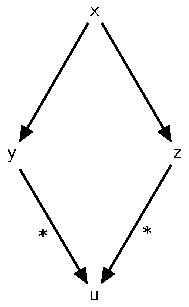
\includegraphics{introduction/example.pdf}
 \caption[Example placeholder figure with a citation~\cite{Higgs:1964ia} and shorter List of Figures caption.
  The List of Figures is protected from first use of glossary entries or acronyms like \acrlong{LHC}.]{%
  This is a placeholder figure to act as an example.
  Here we cite a new reference in the caption to demonstrate that given the package configuration our order of references will not be distributed by the table of contents~\cite{Higgs:1964ia}.}\label{fig:test_figure}
\end{figure}

As can be seen in \Cref{fig:subfigure_example}, the subfigures are independent of each other such that \Cref{fig:subfigure_1} and \Cref{fig:subfigure_2} can be accessed separately.

\begin{figure}[htbp]
 \centering
 \begin{subfigure}[t]{0.48\textwidth}
  \centering
  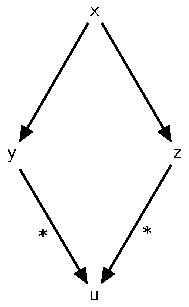
\includegraphics[width=0.3\textwidth]{introduction/example.pdf}
  \caption[Short List of Figures captions work with subfigures too.]{%
   This is the first figure of two, in this example, and its own independent subfigure.}
  \label{fig:subfigure_1}
 \end{subfigure}%
 \quad
 \begin{subfigure}[t]{0.48\textwidth}
  \centering
  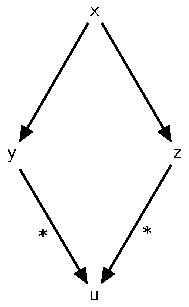
\includegraphics[width=0.3\textwidth]{introduction/example.pdf}
  \caption[Which makes the List of Figures readable and actually helpful.]{%
   As the \texttt{t} alignment option was chosen for the subfigures, they are still properly aligned vertically even though this caption is longer.}
  \label{fig:subfigure_2}
 \end{subfigure}
 \caption{An example of a figure that consists of two subfigures.}
 \label{fig:subfigure_example}
\end{figure}

As an example of an equation formatted in ``\href{https://www.overleaf.com/learn/latex/Display_style_in_math_mode}{display style}'' the equation for the fiducial cross section from~\cite{Aaboud:2016mmw} is reproduced as \Cref{eq:fiducial_cross_section}:
\begin{equation}
 \sigma_{\mathrm{inel}}^{\mathrm{fid}} \left(\zeta > 10^{-6}\right) = \frac{N - N_{\mathrm{BG}}}{\epsilon_{\mathrm{trig}} \times \mathcal{L}} \times \frac{1 - f_{\zeta < 10^{-6}}}{\epsilon_{\mathrm{sel}}}
 \label{eq:fiducial_cross_section}
\end{equation}

\section{Creating Tables}\label{sec:tables}

To create tables in \LaTeX{} it is highly recommended to use the \href{https://www.ctan.org/pkg/booktabs}{\texttt{booktabs}} package.
It allows for very elegant and clean table creation, such as \Cref{table:natural_units}.
If you want to create a table quickly, or have a CSV file that you'd like to quickly turn into a table there are various \href{https://www.tablesgenerator.com/}{online \LaTeX{} table generators}.

\begin{table}[htpb]
 \centering
 \caption[Common quantities in particle physics in natural and SI units.]{%
  Common quantities in particle physics given in both natural units and SI units.}
 \begin{tabular}{@{}llll@{}} \toprule
  Quantity         & Natural Units                 & Natural Units (dimensionful)            & SI Units                                              \\ \midrule
  Speed            & $1$                           & $c$                                     & $3.0\times 10^{8}~\mathrm{m}/\mathrm{s}$              \\
  Angular Momentum & $1$                           & $\hbar$                                 & $10^{34}~\mathrm{m}^2 \,\mathrm{kg}/\mathrm{s}$       \\
  Energy           & $\mathrm{GeV}$                & $\mathrm{GeV}$                          & $1.6\times 10^{-10}~\mathrm{J}$                       \\
  Momentum         & $\mathrm{GeV}$                & $\mathrm{GeV}/c$                        & $1\times 10^{-19}~\mathrm{kg}\,\mathrm{m}/\mathrm{s}$ \\
  Mass             & $\mathrm{GeV}$                & $\mathrm{GeV}/c^{2}$                    & $1.8\times 10^{-27}~\mathrm{kg}$                      \\
  Time             & $1/\mathrm{GeV}$              & $\hbar/\mathrm{GeV}$                    & $6.6\time 10^{-25}~\mathrm{s}$                        \\
  Length           & $1/\mathrm{GeV}$              & $\hbar c/\mathrm{GeV}$                  & $2\times 10^{-16}~\mathrm{m}$                         \\
  Electric Charge  & $1$                           & $e/\sqrt{4\pi \alpha_{\mathrm{em}}}$    & $5.3\times 10^{-19}~\mathrm{C}$                       \\
  Magnetic Field   & $\left(\mathrm{GeV}\right)^2$ & $\left(\mathrm{GeV}\right)^2/\hbar c^2$ & $5\times 10^{16}~\mathrm{T}$                          \\
  \bottomrule
 \end{tabular}\label{table:natural_units}%
\end{table}

Good table design requires some thought and work, so it may be worth a look through some examples:
\begin{itemize}
 \item \href{https://tex.stackexchange.com/questions/238503/tip-on-how-to-make-a-visually-good-table}{TeX StackExchange: Tip on how to make a visually good table}
 \item \href{https://twitter.com/edwardtufte/status/451820483109847040?lang=en}{Edward Tufte endorsed} example from \href{http://static1.squarespace.com/static/56713bf4dc5cb41142f28d1f/t/56fd4c83746fb9261146eed5/1459440776291/ClearOffTheTableMd.gif}{Darkhorse Analytics}
\end{itemize}

\section{Dealing with Widows and Orphans}\label{sec:widos_and_orphans}

To reduce the difficulty of dealing with widowed text (the last line of a paragraph at the start of a page) and orphaned text (the first line of paragraph at the end of a page) the \href{https://ctan.org/pkg/nowidow?lang=en}{\texttt{nowidow}} package is used.
However, that doesn't solve the issue of orphaned section titles.
The user must manually do this, but the following \href{https://texfaq.org/FAQ-widows}{simple advice from \TeX{} FAQ} is recommended:

\begin{quote}
 Once you've exhausted the automatic measures, and have a final draft you want to ``polish'', you should proceed to manual measures.
 To get rid of an orphan is simple: precede the paragraph with \texttt{\textbackslash clearpage} and the paragraph can’t start in the wrong place.
\end{quote}


\chapter{Introduction}\label{chapter:introduction}

%The basic structure of every lab report you've ever done is: 
%    introduction,
%    theory,
%    experimental setup,
%    procedure,
%    results,
%    conclusion.
%
%This thesis is essentially following that same format:
%    Introduction,
%    Standard Model... and Signal modelling? (theory),
%    LHC and ATLAS and Trigger (experimental setup)
%    Reconstruction, Selection, Background Estimation (procedure)
%    results (...)
%    conclusion

The Higgs Boson was proposed as a fundamental particle in 1964
    and has been a driving factor in particle physics research ever since.
Though it was jointly discovered in 2012 by the ATLAS and CMS collaborations,
    there are still a number of properties of the Higgs which have yet to be measured.
Chief among these are two of the Higgs' self-coupling constants
    that determine how strongly the Higgs interacts with both itself and with vector bosons.
The unknown quality of these constants is represented in this analysis by a set of scaling factors, \kl and \kvv,
    which multiply the coupling constants from their expected Standard Model value.
This analysis performs a search for the rare,
    as-yet unseen di-Higgs interaction in order to observe -- or,
    failing observation, to set tighter constraints -- on these scaling values.
The search utilizes the Vector Boson Fusion (VBF) production mechanism of the di-Higgs process,
    wherein two incoming quarks emit a pair of vector bosons that fuse into some intermediate state
    as the initial quarks continue along deflected trajectories.
The di-Higgs system is identified in its four bottom quark ($b \bar b b \bar b$) decay mode,
    producing a minimum 6-jet final state.
This is performed using 126 $\textrm{fb}^{-1}$ of data from Run 2 of ATLAS.

This thesis will begin by first explaining the importance of the Higgs Boson to the field of particle physics,
    as well as the relevance of the aforementioned \kl and \kvv scaling factors.
I will then describe the physical effects of these constants,
    and how those effects can be exploited in order to make measurements of them.
These topics comprise Chapter \ref{chapter:theory}.
Following from the theoretical discussion,
    I will discus the experimental equipment and setup used to perform these measurements across three chapters.
Chapter \ref{chapter:lhc} discusses the Large Hadron Collider, the machine that generates the conditions necessary to produce the di-Higgs process.
Actual observation of the process once generated is carried out by the ATLAS particle detector array and its Trigger system,
    described in Chapters \ref{chapter:atlas} and \ref{chapter:data}.
The reconstruction process, described in Chapter \ref{chapter:reconstruction},
    entails how data observed by ATLAS are analyzed in order to determine which physics processes occurred during the myriad observed interactions.
Background processes are removed from the data set using a selection procedure explained in Chapter \ref{chapter:selection},
    and the contribution of the remaining background events is estimated using a data-driven technique explained in Chapter \ref{chapter:background}. 
The background estimation process makes use of a neural network reweighting procedure, which I personally configured and trained.
My primary contribution to the analysis however, comes in the form of the signal model that constitutes the hypothesis for the behavior of the Higgs Boson.
The signal model makes use of a Monte-Carlo sample combination technique that I developed and optimized in the context of the \vbfproc process.
This is elaborated upon in Chapter \ref{chapter:signal}.
Finally, in Chapter \ref{chapter:results}, this hypothesis and the background estimate are compared against the data observed from ATLAS,
    in order to make constraints on the di-Higgs self-coupling constants.


